\section{Versuchsaufbau/-durchführung}

\subsection{Versuchsaufbau}
Der Versuchsaufbau ist in Abbildung \ref{fig: versuchsaufabu} dargestellt.
Zusehen sind neben dem Zählrohr auch die Messapparatur.   %und die nachgeschaltete Elektronik klingt blöd
Die Messapparatur umfasst einen Verstärker, ein Oszilloskop und
ein Zählwerk. Das Zählwerk gibt die Anzahl der eintreffenden Teilchen
an. Der nach dem Zählrohr geschaltete Kondensator $C$ koppelt den eintreffenden
Stromimpuls vom Zählrohr ab.
\begin{figure}
  \centering
  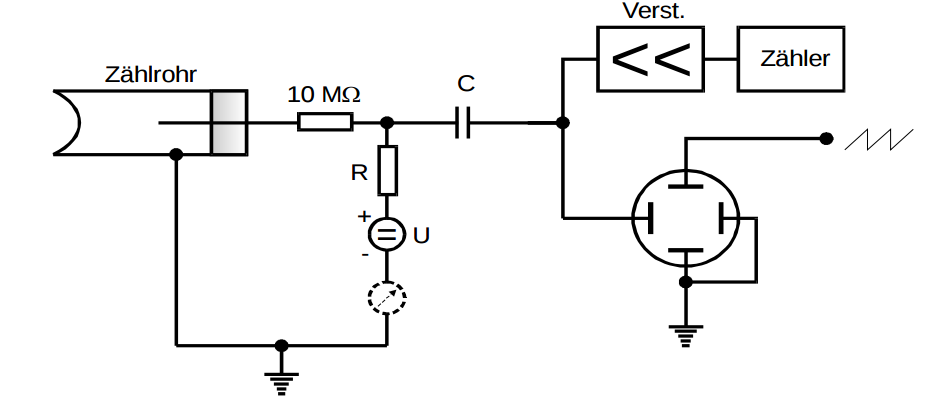
\includegraphics[width=0.6\textwidth]{bilder/aufbau.png}
  \caption{Schematische Darstellung des Aufbaus für die Untersuchung eines Geiger-Müller-Zählrohrs \cite{anleitung703}.}
  \label{fig: versuchsaufabu}
  \end{figure}
\subsection{Versuchsdurchführung}

\subsubsection{Aufnahme der Charakteristika des Zählrohrs} %s.o.

Nachdem eine $\beta$-Quelle vor das Fenster des Zährohrs platziert wurde,
kann die Zählrate in Abhängigkeit von der Betriebsspannung $U$ gemessen werden.
Es werden Zählraten für den Bereich $U\in\left[300, 700\right] \, \si{\volt}$
untersucht. Eine Messung umfasst einen Zeitraum von $\SI{60}{\second}$.


\subsubsection{Oszillographische Messung Tot- und Erholungszeit} %Oszillographische
Man schließt zunächst das Geiger-Müller-Zählrohr an ein
Oszilloskop an. Das Oszilloskop zeigt nun den in Abbildung \ref{fig: totzeit}
dargestellten Spannungsverlauf an. Mit einer geeigneten Zeitskalierung am Oszilloskop
kann die Tot- und Erholungszeit abgelesen werden.
\begin{figure}
  \centering
  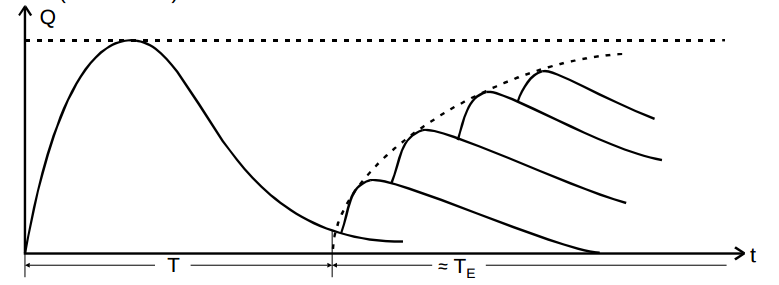
\includegraphics[width=0.6\textwidth]{bilder/totzeit.png}
  \caption{Tot- und Erholungszeit von einem Geiger-Müller-Zähler \cite{anleitung703}.}
  \label{fig: totzeit}
  \end{figure}
Die Prozedur wird für fünf verschiedene Spannungen durchgeführt.

\subsection{Bestimmung der Totzeit mit der Zwei-Quellen-Methode}
Auf Grund der Totzeit $T$ eines Geiger-Müller-Zähler, gibt es immer einen
Unterschied zwischen der realen und der gemessenen Zählrate. %wahr unphysikalisch
Der Zusammenhang zwischen der gemessenen Zählrate $N\ua{r}$ und
realen $N\ua{w}$ lautet: %s.o.
\begin{equation}
  \label{eq:wahre_zaehlrate}
  N\ua{w}=\frac{N\ua{r}}{1-TN\ua{r}}.
\end{equation}
Die Verwendung zweier unterschiedlicher Präparate bietet eine Möglichkeit zur %zweier unterschiedlicher; zur
Bestimmung der Totzeit. Dazu wird bei $\SI{480}{\volt}$ und in einem Zeitraum von $\SI{60}{\second}$ eine neue %einem Zeitraum von
$\ce{^{204}Tl}$ und einer alte $\ce{^{204}Tl}$ Probe untersucht.
Auf Grund der Halbwertszeit besitzt die alte $\ce{^{204}Tl}$ Probe eine geringere
Strahlungsintensität als die neue Probe und kann so für die Zwei-Quellen-Methode verwendet
werden.  %kurz erwähnen warum
Zunächst wird die Zählrate $N_1$ einer Probe bestimmt, danach die %leerzeichen
Summe aus beiden $N_1+N_2$. Beim Einsetzen der zweiten Probe darf die Position der
ersten Probe nicht verändert werden.
Abschließend wird die erste Probe entfernt und die Zählrate $N_2$ für die zweite
Probe notiert.
Auf Grund der Totzeit gilt der Zusammenhang
\begin{equation}
  \label{eq:totzeit_summe}
  N_{1+2}<N_1+N_2,
\end{equation}
mit diesem kann dann die Totzeit gemäß %gemäß
\begin{equation}
  \label{eq:totzeit}
  T\approx \frac{N_1+N_2-N_{1+2}}{2N_1N_2}
\end{equation}
genährt werden.

\subsubsection{Messung der pro Teilchen vom Zählrohr feigesetzten Ladundsmenge} %freigesetzten Ladungsmenge
Die vom eindringenden Teilchen im Zählrohr freigesetzte Ladungsmenge kann mit
\begin{equation}
  \label{eq:lafung_pro_teilchen}
  I=\frac{\Delta Q}{\Delta t} N
\end{equation}
berechnet werden ($N$ ist die Anzahl der Teilchen).
Mit Hilfe eines empfindlichen Strommessgerätes
kann die Ladungsenge in Abhängigkeit von der Spannung $U$ untersucht werden.
Der für den Versuch gewählte Spannungsbereich liegt bei $U\in\left[300, 700\right] \, \si{\volt}$.
